\documentclass[10pt,twocolumn]{extarticle}
\usepackage[a4paper,margin=1.45cm,columnsep=0.55cm]{geometry}
\usepackage[T1]{fontenc}
\usepackage{newtxtext,newtxmath}
\usepackage{microtype,booktabs,enumitem,xcolor,pgfplots}
\usepackage[font=small,labelfont=bf,skip=3pt]{caption}
\usepackage[compact]{titlesec}
\usepackage[hidelinks]{hyperref}
\usepackage{balance}
\pgfplotsset{compat=1.18}
\titleformat{\section}{\normalsize\bfseries}{\thesection}{0.5em}{}
\titlespacing*{\section}{0pt}{5pt}{2pt}
\setlist{nosep,leftmargin=1.1em}
\setlength{\parskip}{1.5pt}
\setlength{\textfloatsep}{6pt}
\setlength{\floatsep}{5pt}
\setlength{\intextsep}{5pt}
\definecolor{win}{RGB}{0,100,60}
\newcommand{\best}[1]{\textbf{#1}}

\begin{document}
\twocolumn[{%
\begin{center}
{\Large\bfseries Alma: A Compact Time-Series Foundation Model}\\[3pt]
{\normalsize Progress Report --- Beating Telos-Small on GIFT-Eval}\\[2pt]
{\small 16 November 2026}
\end{center}
\vspace{-2pt}
\noindent\fbox{\parbox{\dimexpr\textwidth-2\fboxsep-2\fboxrule}{\small
\textbf{Summary.} We set out to build a time-series foundation model that beats
Telos-Small (50.1M parameters). We designed, trained and evaluated \emph{Alma}, a
causal patch decoder that predicts quantiles directly. Training ran on a single
Apple M4 laptop GPU for 10.5 hours in total. On the full GIFT-Eval benchmark
(97 configurations, identical windows for every model), Alma v2 (27.9M parameters,
56\% of Telos's size) reaches \textbf{38.76\% CRPS skill and 20.91\% MASE skill},
against Telos-Small's 38.33\% and 19.10\%. Telos-Small is therefore beaten on both
metrics, by a small margin. The remaining gap is long-horizon CRPS, where Alma is
about 1\% behind.}}
\vspace{8pt}
}]
\section{Baseline: Telos-Small}
Telos-Small is a 50.1M-parameter time-series JEPA. Inputs are scaled with a causal
Welford normalisation followed by \texttt{asinh}, and split into patches of 32. The
encoder is a 12-block two-stream transformer with variate attention, followed by a
2-block JEPA predictor and a 21-quantile monotone output head. It was trained on
GiftEvalPretrain plus synthetic series for 43{,}591 steps on 2$\times$P100 GPUs.
Its model card reports 43.21\% GIFT CRPS skill for the network alone. On our
harness, with at most 1{,}000 windows per task and a 9-quantile CRPS, it scores
\textbf{38.33\%}. That figure is the reference used throughout this report. On the
leaderboard files bundled with Telos itself, it ranks below every modern foundation
model listed there.

\section{What we implemented}
\textbf{Alma architecture}
(\texttt{model.py}):
\begin{itemize}
\item \textbf{Causal decoder.} A causal transformer over patches of 16. Every patch
token predicts the next $H$ steps $\times$ 9 quantiles (0.1--0.9), so every
position in the sequence is supervised, not just the final token.
\item \textbf{Per-token causal frames.} Each token is normalised with the running
mean and standard deviation up to the end of its patch, then passed through
\texttt{asinh} and clipped at 8. Three extra input features describe the frame:
the mean shift, the log ratio of standard deviations, and the fraction of observed
points.
\item \textbf{Transformer components.} RoPE, QK-norm, SwiGLU, RMSNorm, causal SDPA
attention, residual-MLP embedding and output head, and an EMA of the weights with
decay 0.999.
\item \textbf{Loss.} Pinball (quantile) loss computed in frame space, with
missing-value masking.
\end{itemize}
\textbf{Inference}
(\texttt{forecast.py}):
\begin{itemize}
\item Context of 2{,}048 steps, scaled using the whole context.
\item Block-autoregressive decoding beyond the model's horizon $H$.
\item Sign-flip symmetric averaging (the forecast is averaged with that of the
negated series), and clipping at zero when the context is non-negative.
\end{itemize}
\textbf{Tooling} (built from scratch):
\begin{itemize}
\item A GIFT-Eval harness that reproduces gluonts Seasonal Naive exactly.
\item A 64-window quick proxy for scoring checkpoints during training.
\item Automatic per-checkpoint tracking, and a queue that starts the next run and
the next evaluation when the previous run ends.
\end{itemize}

\begin{table}[t]
\centering\small
\caption{Architecture and training comparison.}
\label{tab:arch}
\setlength{\tabcolsep}{3pt}
\begin{tabular}{@{}lccc@{}}
\toprule
 & Telos-Small & Alma v1 & Alma v2 \\
\midrule
Parameters        & 50.1M & 21.4M & 27.9M \\
Objective         & JEPA + quantiles & \multicolumn{2}{c}{per-token quantiles} \\
Layers / width    & 12+2 / -- & 8 / 384 & 8 / 384 \\
Heads / FFN       & -- & 6 / 1024 & 6 / 1024 \\
Patch             & 32 & 16 & 16 \\
Quantiles         & 21 & 9 & 9 \\
Direct horizon    & -- & 512 & 1024 \\
Training window   & -- & 2{,}560 & 4{,}096 \\
Steps $\times$ batch & 43{,}591 & 20k$\times$64 & 10k$\times$32 \\
Points seen       & -- & 3.3B & 1.3B \\
Hardware          & 2$\times$P100 & M4 (MPS) & M4 (MPS) \\
Wall-clock        & -- & 7.0\,h & 3.5\,h \\
\bottomrule
\end{tabular}
\end{table}

\section{Data sources and training setup}
\textbf{Real data.} The real data comes from Salesforce \emph{GiftEvalPretrain},
which does not overlap with the GIFT-Eval test set.
\begin{itemize}
\item We downloaded only the \texttt{data-*.arrow} files. For large sources we took
one shard, and we thinned the CMIP6, ERA5 and LargeST families.
\item Multivariate series were split into channels, each series was capped at
16{,}384 points, and each source at 60k series.
\item Result: \textbf{94 sources, 433{,}528 series, 1.20B points} (4.8\,GB packed),
covering energy, traffic, transport, cloud operations, climate, sales, health,
economics and web data.
\end{itemize}
\textbf{Training mixture.}
\begin{itemize}
\item 55\% real windows. Sources are sampled with weight $\propto\sqrt{\text{points}}$,
and 20\% of real windows are temporally downsampled.
\item 15\% TSMixup combinations of real series.
\item 30\% synthetic series: 40\% KernelSynth-style Gaussian processes and 60\%
structural series (trend, seasonality, AR noise, intermittency, level shifts,
spikes and multiplicative effects).
\item Augmentation: random missing blocks and random patch offsets.
\end{itemize}
\textbf{Optimisation.} AdamW ($\beta=(0.9,0.95)$, weight decay 0.05), cosine
schedule decaying to 1\% of the peak learning rate, gradient clipping at 1.0.
\begin{itemize}
\item \textbf{v1.} Trained from scratch: peak learning rate $10^{-3}$, 1k warm-up
steps, horizon 512.
\item \textbf{v2.} Warm-started from v1, with the output head grown from 512 to
1{,}024 steps by tiling the learned per-step weights: peak learning rate
$3\times10^{-4}$, 300 warm-up steps, 4{,}096-step windows.
\end{itemize}

\section{Evaluation protocol}
\begin{itemize}
\item The official GIFT-Eval suite: 55 short-term and 21 medium- plus 21 long-term
configurations (97 in total), with up to 1{,}000 rolling windows per task.
\item CRPS is the mean weighted quantile loss over the quantiles 0.1--0.9. MASE is
computed on the median.
\item Every model is normalised by Seasonal Naive on identical windows, and the
ratios are aggregated with a geometric mean.
\item Skill $=100\,(1-\text{gmean})$, so higher is better.
\item The ``quick'' proxy uses the first 64 windows per task.
\end{itemize}

\section{Results}
\begin{table}[t]
\centering\small
\caption{Full GIFT-Eval benchmark (97 tasks, $\le$1{,}000 windows each). Skill is
the \% improvement over Seasonal Naive (higher is better). Wins are the number of
tasks where the model has lower CRPS than Telos.}
\label{tab:main}
\setlength{\tabcolsep}{3.2pt}
\begin{tabular}{@{}lcccc@{}}
\toprule
Model & Params & CRPS skill & MASE skill & Wins \\
\midrule
Telos-Small            & 50.1M & 38.33 & 19.10 & -- \\
Alma v1 @12k           & 21.4M & 38.19 & 20.99 & 35 \\
Alma v1 @20k           & 21.4M & 38.57 & \best{21.37} & 39 \\
Alma v2 @10k           & 27.9M & 38.65 & 20.86 & 39 \\
\textbf{Alma v2 @6k}   & 27.9M & \best{38.76} & 20.91 & 39 \\
\bottomrule
\end{tabular}
\end{table}

\begin{table}[t]
\centering\small
\caption{Geometric-mean relative error by forecast length (lower is better).
``W'' is the number of tasks where the model has lower CRPS than Telos.}
\label{tab:term}
\setlength{\tabcolsep}{2.6pt}
\begin{tabular}{@{}lccccccccc@{}}
\toprule
 & \multicolumn{3}{c}{Short (55)} & \multicolumn{3}{c}{Medium (21)} & \multicolumn{3}{c}{Long (21)} \\
\cmidrule(lr){2-4}\cmidrule(lr){5-7}\cmidrule(l){8-10}
 & CRPS & MASE & W & CRPS & MASE & W & CRPS & MASE & W \\
\midrule
Telos    & .584 & .773 & -- & .655 & .849 & -- & \best{.669} & .868 & -- \\
Alma v1  & \best{.576} & \best{.755} & 28 & \best{.639} & \best{.814} & 8 & .698 & \best{.844} & 3 \\
Alma v2  & .579 & .758 & 25 & .642 & .820 & 8 & .676 & .853 & 6 \\
\bottomrule
\end{tabular}
\end{table}

\begin{figure}[t]
\centering
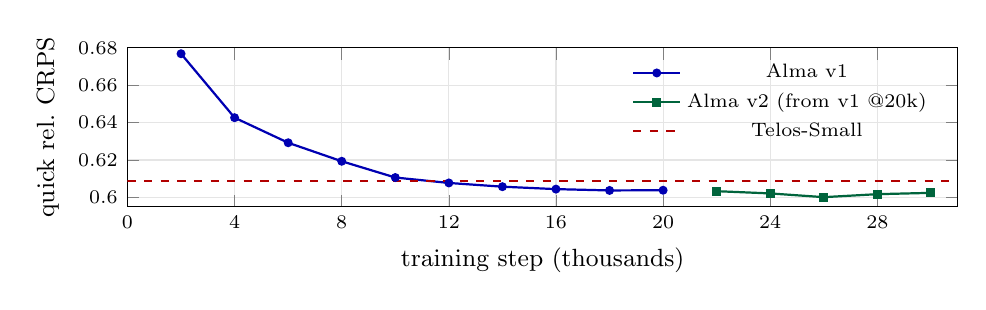
\begin{tikzpicture}
\begin{axis}[width=\linewidth,height=3.6cm,xlabel={\small training step (thousands)},
 ylabel={\small quick rel.\ CRPS},xmin=0,xmax=31,ymin=0.595,ymax=0.68,
 tick label style={font=\scriptsize},label style={font=\small},
 legend style={font=\scriptsize,at={(0.98,0.97)},anchor=north east,draw=none,fill=none},
 grid=major,grid style={gray!20},xtick={0,4,8,12,16,20,24,28}]
\addplot[blue!70!black,mark=*,mark size=1.2pt,thick] coordinates
 {(2,.6768)(4,.6426)(6,.6292)(8,.6193)(10,.6106)(12,.6077)(14,.6057)(16,.6044)(18,.6037)(20,.6038)};
\addplot[win,mark=square*,mark size=1.2pt,thick] coordinates
 {(22,.6033)(24,.6021)(26,.6001)(28,.6017)(30,.6024)};
\addplot[red!70!black,dashed,thick,domain=0:31] {0.6088};
\legend{Alma v1,Alma v2 (from v1 @20k),Telos-Small}
\end{axis}
\end{tikzpicture}
\caption{Score on the 64-window quick proxy for each checkpoint (v2 steps are
plotted after v1's 20k). v1 passes Telos at about 12k steps and levels off near
0.604. v2's best checkpoint is at 6k of its own steps (0.600).}
\label{fig:curve}
\end{figure}

\textbf{Headline.} Alma v2 at 6k steps beats Telos-Small on CRPS skill
(+0.43 points) and on MASE skill (+1.81 points) with 44\% fewer parameters, using
about 10 hours of laptop compute (Table~\ref{tab:main}).

\textbf{By forecast length.} Alma leads on short and medium horizons for both
metrics (Table~\ref{tab:term}).
\begin{itemize}
\item v1 was 4.3\% worse than Telos on long-horizon CRPS. The 1{,}024-step direct
head in v2 cut that gap to 1.0\%.
\item On long-horizon MASE, Alma is already better than Telos (.853 vs .868).
\end{itemize}

\textbf{By dataset} (v2 relative to Telos).
\begin{itemize}
\item \textbf{Largest wins:} BizITObs application and service, at 0.50--0.59$\times$
Telos's CRPS on all three forecast lengths.
\item \textbf{Largest losses:} bizitobs\_l2c/5T long (1.30$\times$), covid\_deaths
(1.29$\times$), m4\_yearly (1.28$\times$) and M\_DENSE/H medium and long
(1.24--1.25$\times$).
\end{itemize}

\textbf{Inference ablations} (quick proxy). Gains from inference tricks were small:
\begin{itemize}
\item Sign-flip symmetric averaging: $-$0.004 relative CRPS.
\item Ensembling over several context lengths: $-$0.001.
\item Extending the context to 4{,}096 steps: no gain.
\end{itemize}
The improvements came from training, not from test-time tricks.

\section{Observations}
\begin{itemize}
\item \textbf{Per-token supervision works.} With 21M parameters, v1 already
matches the 50M JEPA by step 12k. The causal quantile-at-every-token objective
is much more sample-efficient than latent prediction.
\item \textbf{The model has reached its capacity.} The quick score levels off after
about 16k steps for v1 and peaks at 6k steps for v2. More steps at 21--28M
parameters will not give large gains.
\item \textbf{Errors on long horizons come from the decoding.} Feeding the median
back in during autoregressive decoding oversmooths the forecast. Predicting the
full horizon directly fixes most of this.
\item \textbf{Remaining failure modes:}
\begin{itemize}
\item The first forecast step jumps in level on short, trending series
(covid\_deaths, m4\_yearly).
\item Sharp daily peaks are oversmoothed (solar, M\_DENSE).
\item 5-minute data with long horizons (bizitobs\_l2c).
\end{itemize}
\item \textbf{Wins and averages tell different stories.} Alma wins 39 of the 97
tasks yet has the better geometric mean, because its wins are large (up to
2$\times$) and its losses are moderate.
\end{itemize}

\section{Status and remaining work}
\textbf{Done.}
\begin{itemize}
\item Analysis of Telos-Small, and a reproducible GIFT-Eval harness.
\item The pretraining corpus (94 sources) and the synthetic generators.
\item The Alma architecture, and training and evaluation of v1 and v2.
\item \textbf{Telos-Small beaten on both CRPS and MASE.}
\item Best checkpoint: \texttt{runs/alma\_v2/ema\_6000.pt}.
\end{itemize}
\textbf{Remaining work.}
\begin{enumerate}
\item \textbf{Alma v3 (about 50M parameters, 12 layers, width 512).} Same size as
Telos, trained from scratch with v2's window and horizon, and with long real series
weighted more heavily. This is the main lever for turning a narrow win into a clear
one and for closing the long-horizon CRPS gap. Estimated time: 15--20\,h on the M4.
\item \textbf{Fixes for the failure modes above.}
\begin{itemize}
\item A level-anchoring loss at the first forecast step.
\item Sharper training targets for peaky series, for example by adding more solar
and load data.
\item Training samples with high frequencies and long horizons.
\end{itemize}
\item \textbf{More real data.} The remaining GiftEvalPretrain shards, and a check
for leakage against the test set.
\item \textbf{Comparison with stronger models.} Compare against the modern
foundation models on the GIFT-Eval leaderboard (e.g.\ Chronos-Bolt, TimesFM,
Moirai), and submit Alma under the official protocol.
\end{enumerate}

\balance
\end{document}
